\documentclass[tikz,border=12pt]{standalone}
\usepackage[T1]{fontenc}
\usepackage{mathpazo}
\usepackage{amsmath,amssymb}
\usetikzlibrary{arrows.meta, positioning, calc, fit, decorations.pathreplacing}

\definecolor{stblue}{HTML}{7B97AD}
\definecolor{rwgold}{HTML}{B8995E}
\definecolor{sage}{HTML}{7A9A7E}
\definecolor{dkbrown}{HTML}{3D3530}
\definecolor{wmgray}{HTML}{7B7067}
\definecolor{cream}{HTML}{F9F6F0}
\definecolor{border}{HTML}{D4C9B8}
\definecolor{terracotta}{HTML}{C47A6A}

\begin{document}
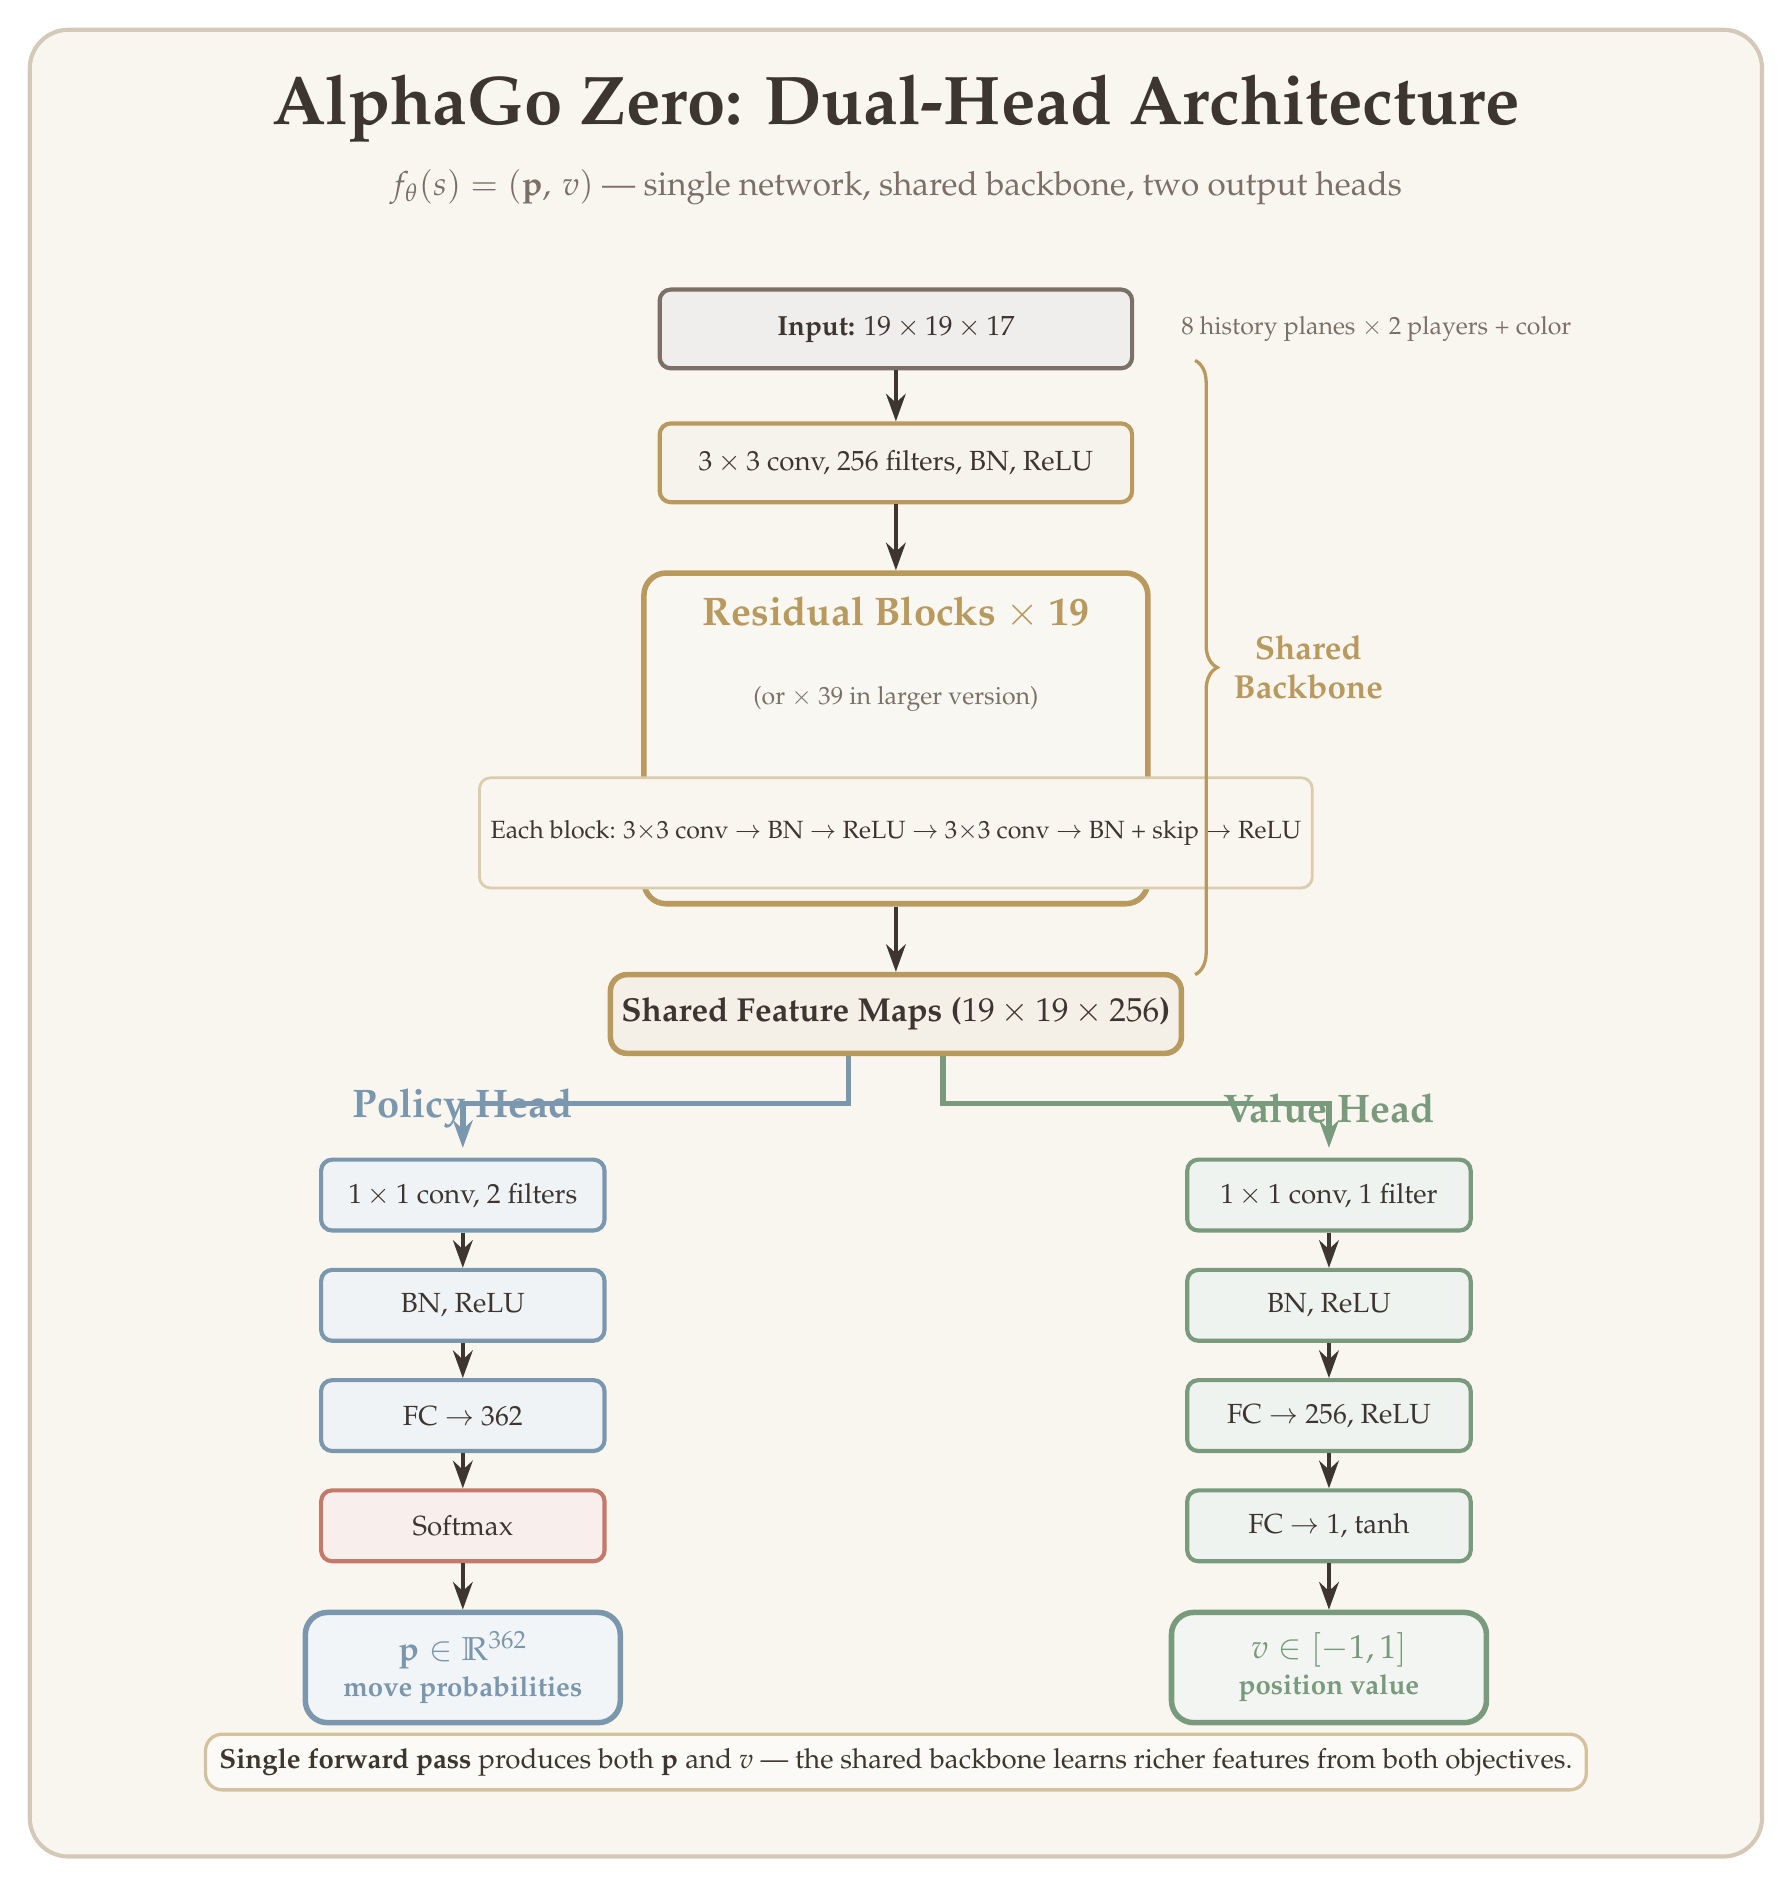
\begin{tikzpicture}[
  >={Stealth[length=3.5mm, width=2.5mm]},
  layer/.style={
    draw=#1, line width=1.5pt, fill=#1!12, rounded corners=4pt,
    minimum width=52mm, minimum height=10mm, font=\normalsize, text=dkbrown,
    align=center, inner sep=3pt
  },
  headlayer/.style={
    draw=#1, line width=1.5pt, fill=#1!12, rounded corners=4pt,
    minimum width=36mm, minimum height=9mm, font=\normalsize, text=dkbrown,
    align=center, inner sep=3pt
  },
  arr/.style={->, line width=1.5pt, dkbrown},
]

% Background
\fill[cream, rounded corners=14pt] (-2,-1.2) rectangle (20,22);
\draw[border, rounded corners=14pt, line width=1.5pt] (-2,-1.2) rectangle (20,22);

% Title
\node[font=\Huge\bfseries, text=dkbrown] at (9,21)
  {AlphaGo Zero: Dual-Head Architecture};

% Subtitle
\node[font=\large, text=wmgray] at (9,20)
  {$f_\theta(s) = (\mathbf{p},\, v)$ --- single network, shared backbone, two output heads};

% =============================================
% Input
% =============================================
\node[layer=wmgray, minimum width=60mm] (input) at (9,18.2)
  {\textbf{Input:} $19 \times 19 \times 17$};
\node[font=\small, text=wmgray, right] at (12.5,18.2)
  {8 history planes $\times$ 2 players + color};

% =============================================
% Shared Backbone (center)
% =============================================

% Initial conv
\node[layer=rwgold, minimum width=60mm] (conv0) at (9,16.5)
  {$3 \times 3$ conv, 256 filters, BN, ReLU};

% Residual blocks
\node[draw=rwgold, line width=2pt, fill=rwgold!8, rounded corners=8pt,
      minimum width=64mm, minimum height=42mm,
      font=\large, text=dkbrown, align=center, inner sep=8pt]
  (resblocks) at (9,13)
  {};

% Content inside res block
\node[font=\Large\bfseries, text=rwgold] at (9,14.6) {Residual Blocks $\times$ 19};
\node[font=\small, text=wmgray, align=center] at (9,13.5) {(or $\times$ 39 in larger version)};

% Single residual block detail
\node[draw=rwgold!50, line width=1pt, fill=cream, rounded corners=4pt,
      minimum width=54mm, minimum height=14mm,
      font=\small, text=dkbrown, align=center, inner sep=4pt]
  at (9,11.8)
  {Each block: $3{\times}3$ conv $\to$ BN $\to$ ReLU $\to$ $3{\times}3$ conv $\to$ BN + skip $\to$ ReLU};

% Shared features output
\node[draw=rwgold, line width=2pt, fill=rwgold!15, rounded corners=6pt,
      minimum width=60mm, minimum height=10mm,
      font=\large\bfseries, text=dkbrown, align=center, inner sep=4pt]
  (shared) at (9,9.5)
  {Shared Feature Maps ($19 \times 19 \times 256$)};

% Arrows for backbone
\draw[arr] (input) -- (conv0);
\draw[arr] (conv0) -- (resblocks);
\draw[arr] (resblocks) -- (shared);

% Brace for shared backbone
\draw[decorate, decoration={brace, amplitude=8pt}, line width=1.2pt, rwgold]
  (12.8,17.8) -- (12.8,10) node[midway, right, xshift=10pt, font=\large\bfseries, text=rwgold, align=center]
  {Shared\\Backbone};

% =============================================
% Split into two heads
% =============================================

% Fork arrows
\draw[arr, stblue, line width=2pt] ([xshift=-6mm]shared.south) -- ++(0,-0.6) -| (3.5,7.8);
\draw[arr, sage, line width=2pt] ([xshift=6mm]shared.south) -- ++(0,-0.6) -| (14.5,7.8);

% =============================================
% LEFT: Policy Head
% =============================================
\node[font=\Large\bfseries, text=stblue] at (3.5,8.3) {Policy Head};

\node[headlayer=stblue] (p-conv) at (3.5,7.2)
  {$1 \times 1$ conv, 2 filters};
\node[headlayer=stblue] (p-bn) at (3.5,5.8)
  {BN, ReLU};
\node[headlayer=stblue] (p-fc) at (3.5,4.4)
  {FC $\to$ 362};
\node[headlayer=terracotta] (p-sm) at (3.5,3.0)
  {Softmax};

% Output
\node[draw=stblue, line width=2pt, fill=stblue!10, rounded corners=8pt,
      minimum width=40mm, minimum height=14mm,
      font=\large\bfseries, text=stblue, align=center, inner sep=5pt]
  (p-out) at (3.5,1.2)
  {$\mathbf{p} \in \mathbb{R}^{362}$\\[-1pt]
   {\normalsize move probabilities}};

\draw[arr] (p-conv) -- (p-bn);
\draw[arr] (p-bn) -- (p-fc);
\draw[arr] (p-fc) -- (p-sm);
\draw[arr] (p-sm) -- (p-out);

% =============================================
% RIGHT: Value Head
% =============================================
\node[font=\Large\bfseries, text=sage] at (14.5,8.3) {Value Head};

\node[headlayer=sage] (v-conv) at (14.5,7.2)
  {$1 \times 1$ conv, 1 filter};
\node[headlayer=sage] (v-bn) at (14.5,5.8)
  {BN, ReLU};
\node[headlayer=sage] (v-fc1) at (14.5,4.4)
  {FC $\to$ 256, ReLU};
\node[headlayer=sage] (v-fc2) at (14.5,3.0)
  {FC $\to$ 1, $\tanh$};

% Output
\node[draw=sage, line width=2pt, fill=sage!10, rounded corners=8pt,
      minimum width=40mm, minimum height=14mm,
      font=\large\bfseries, text=sage, align=center, inner sep=5pt]
  (v-out) at (14.5,1.2)
  {$v \in [-1, 1]$\\[-1pt]
   {\normalsize position value}};

\draw[arr] (v-conv) -- (v-bn);
\draw[arr] (v-bn) -- (v-fc1);
\draw[arr] (v-fc1) -- (v-fc2);
\draw[arr] (v-fc2) -- (v-out);

% =============================================
% Bottom annotation
% =============================================
\node[draw=rwgold!60, line width=1.2pt, fill=rwgold!5, rounded corners=6pt,
      font=\normalsize, text=dkbrown, align=center, inner sep=5pt]
  at (9,0)
  {\textbf{Single forward pass} produces both $\mathbf{p}$ and $v$
   --- the shared backbone learns richer features from both objectives.};

\end{tikzpicture}
\end{document}
